\chapter{Administrátorské rozhraní}
\label{4-praxe}

\begin{figure}[H] \centering
    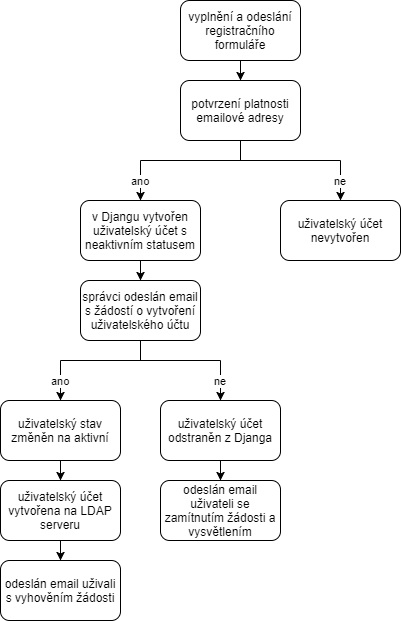
\includegraphics[width=250pt]{./pictures/my_console_final_version_cz.png}
    \caption[Vytváření uživatele - finální stav]{Vytváření uživatele - finální stav (zdroj:
	\href{}{Tereza Kulovaná})}
    \label{fig:admin-final}
  \end{figure}

\begin{figure}[H] \centering
    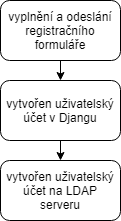
\includegraphics[width=70pt]{./pictures/my_console_current_version_cz.png}
    \caption[Vytváření uživatele - současný stav]{Vytváření uživatele - současný stav (zdroj:
	\href{}{Tereza Kulovaná})}
    \label{fig:admin-current}
  \end{figure}

\section{Současný správa uživatelských účtů}
\label{cmd-line}


\section{Webové administrátorské rozhraní}
spíš z technického hlediska a implementace
(z uživatelského pak jako příloha)

Pro vývoj webové administrátorské konzole byl využit odlehčený webový server Djanga (vývojový server).

\subsection{Struktura projektu}
%popsat strukturu celé aplikace, jednotlivé soubory a třídy
Adresářová struktura projektu:
% tomuhle budu chtít dát hezčí design
% např. forest: https://tex.stackexchange.com/questions/5073/making-a-simple-directory-tree
% https://tex.stackexchange.com/questions/328886/making-a-directory-tree-of-folders-and-files/328890
\dirtree{%
.1 web\_admin\_console.			
	.2 project.
		.3 \_\_init\_\_.py.
		.3 ldap\_auth.py.
		.3 settings.py.
		.3 settings\_custom.py.
		.3 urls.py.
		.3 wsgi.py.
    .2 static.
    	.3 styles.css.
	.2 templates.
		.3 registration.
			.4 login.html.
		.3 base.html.
		.3 home.html.
		.3 password\_change.html.
		.3 signup.html.
		.3 user\_change.html.
	.2 users.
		.3 templatetags.
			.4 \_\_init\_\_.py.
			.4 auth\_extras.py.
		.3 \_\_init\_\_.py.
		.3 admin.py.
		.3 apps.py.
		.3 forms.py.
		.3 ldap\_sync.py.
		.3 models.py.
		.3 tests.py.
		.3 urls.py.
		.3 views.py.
	.2 db.sqlite3.
	.2 manage.py.
    }
% popsat jen ty nejdůležitější soubory


\subsubsection{project}

\subsubsection{templates}
Složka \textit{templates} obsahuje šablony, psané v \zk{HTML}, které umožňují vypisovat vybraná data z modelů do prohlížeče. Cesta k adresáři musí být registrována v souboru \texttt{settings.py} v hodnotě \texttt{DIRS} u položky \texttt{TEMPLATES}.

{{ variables }}
{{ variable|filter }}
- custom templatetags

popsat zbylá html

Django funguje na principu dědičnosti. Bázovou šablonou je \textit{base.html}. Vložením textu \texttt{\{\% extends "base.html" \%\}} na začátek jiné šablony, např. \textit{child.html}, je nejdříve načtena šablona \textit{base.html}, definující základní bloky, a až následně je k nim přidán obsah \textit{child.html}. Tímto způsobem jsou sníženy duplicity v jednotlivých šablonách. 

Složka \textit{static} umístěná v hlavním adresáři projektu obsahuje soubor \textit{styles.css}, který popisuje způsob zobrazení elementů, které jsou součástí jednotlivých šablon uživatelské konzole. To je umožněno načtením tohoto souboru pomocí \texttt{\{\% load static \%\}} do bázové šablony. K vytvoření designu byly použity kaskádové style (\zk{CSS}).

\subsubsection{users}

\subsubsection{db.sqlite3}
% https://www.tablesgenerator.com/latex_tables

Pro vývoj byla využita implicitní databáze Djanga SQLite. 
Z hlediska uživatelů a rolí jsou důležité především tři tabulky \textit{auth\_group}, \textit{users\_customuser} a \textit{users\_customuser\_groups}. 

Tabulka \textit{auth\_group} obsahuje pouze názvy existujících rolí.

\begin{table}[H]
\centering
\begin{tabular}{@{}|c|c|c|@{}}
\toprule
\multicolumn{3}{|c|}{auth\_group} \\ \midrule
name & id & name \\ \midrule
type & integer & varchar(80) \\ \bottomrule
\end{tabular}
\caption{Atributy tabulky auth\_group}
\label{tab:auth-group}
\end{table}

Tabulka \textit{users\_customuser} sestává z osobních údajů uživatelů včetně zašifrovaného hesla, data vytvoření, posledního přihlášení a interních statusů Djanga. 

\begin{table}[H]
\centering
\resizebox{\textwidth}{!}{%
\begin{tabular}{@{}|c|c|c|c|c|c|c|@{}}
\toprule
\multicolumn{7}{|c|}{users\_customuser} \\ \midrule
name & id & password & last\_login & is\_superuser & username & first\_name \\ \midrule
type & integer & varchar(128) & datetime & bool & varchar(150) & varchar(30) \\ \bottomrule
\end{tabular}%
}
\caption{Atributy tabulky users\_customuser 1/2}
\label{tab:users-customuser-1}
\end{table}

\begin{table}[H]
\centering
\resizebox{\textwidth}{!}{%
\begin{tabular}{@{}|c|c|c|c|c|c|c|@{}}
\toprule
\multicolumn{7}{|c|}{users\_customuser} \\ \midrule
name & last\_name & email & is\_staff & is\_active & date\_joined & description \\ \midrule
type & varchar(150) & varchar(254) & bool & bool & datetime & text \\ \bottomrule
\end{tabular}%
}
\caption{Atributy tabulky users\_customuser 2/2}
\label{tab:users-customuser-2}
\end{table}

Tabulka \textit{users\_customuser\_groups} propojuje obě výše zmíněné tabulky, tj. příslušnost uživatelů k jednotlivým skupinám.

\begin{table}[H]
\centering
\begin{tabular}{@{}|c|c|c|c|@{}}
\toprule
\multicolumn{4}{|c|}{users\_customuser\_groups} \\ \midrule
name & id & customuser\_id & group\_id \\ \midrule
type & integer & integer & integer \\ \bottomrule
\end{tabular}
\caption{Hlavička tabulky users\_customuser\_groups}
\label{tab:users-customuser-groups}
\end{table}

\subsection{problémy při zpracování}

\subsection{co přibude do budoucna}
\label{python-knihovna}


